% !TEX encoding = UTF-8 Unicode 
\documentclass[9pt, aspectratio=169, xcolor=table]{beamer}
\setbeamercovered{transparent=10}
\usetheme[
%  showheader,
  colorblocks,
%  noframetitlerule,
]{Verona}
\definecolor{deepbullblue}{rgb}{0,0.298, 0.427}
\definecolor{sunbeltyellow}{rgb}{1,0.792, 0.024}
\definecolor{redbullred}{rgb}{0.8,0.122, 0.294}
\definecolor{mGreen}{rgb}{0,0.6,0}
\definecolor{mGray}{rgb}{0.5,0.5,0.5}
\definecolor{grissuave}{rgb}{0.25,0.25,0.25}
\definecolor{mPurple}{rgb}{0.58,0,0.82}
\definecolor{backgroundColour}{rgb}{0.95,0.95,0.92}

\definecolor{alizarin}{rgb}{0.82, 0.1, 0.26}
\definecolor{ao}{rgb}{0.0, 0.5, 0.0}

\usepackage{minted}
\usepackage{svg}
\usepackage{listings}

\usepackage[spanish,es-tabla]{babel}

\lstdefinestyle{CStyle}{
    backgroundcolor=\color{backgroundColour},   
    commentstyle=\color{mGreen},
    keywordstyle=\color{magenta},
    numbers=none,
    %numberstyle=\tiny\color{mGray},
    %numbers=left,                    
    %numbersep=5pt,                  
    stringstyle=\color{mPurple},
    basicstyle=\ttfamily,
    breakatwhitespace=false,         
    breaklines=true,                 
    captionpos=b,                    
    keepspaces=true,                 
    showspaces=false,
    columns=fixed,
    showstringspaces=false,
    showtabs=false,                  
    tabsize=2,
    language=C
}

\usepackage[T1]{fontenc}
\usepackage[utf8]{inputenc}
\usepackage{listings}
\usepackage{datetime}
\usepackage{lipsum}
\usepackage{todonotes}
\usepackage[export]{adjustbox}
%\usepackage[spanish,onelanguage,boxed, boxruled, algoruled]{algorithm2e}
%\usepackage[spanish,onelanguage,boxed, algoruled]{algorithm2e}
%\usepackage{algcompatible}
\usepackage{algorithm}
\usepackage[noend]{algpseudocode}
%%%%%%%%%%%%%%%%%%%%%%%%%%%%%%%
% Mac上使用如下命令声明隶书字体,windows也有相关方式,大家可自行修改
%\providecommand{\lishu}{\CJKfamily{zhli}}
%%%%%%%%%%%%%%%%%%%%%%%%%%%%%%%
\usepackage{tikz}
\usetikzlibrary{fadings}
%
%\setbeamertemplate{sections/subsections in toc}[ball]
%\usepackage{xeCJK}
\usepackage{caption}
\usepackage{subcaption}
\usefonttheme{professionalfonts}
\def\mathfamilydefault{\rmdefault}
\usepackage{amsmath}
\usepackage{multirow}
\usepackage{booktabs}
\usepackage{multicol}
\usepackage{bm}

\def\testclr#1#{\@testclr{#1}}
%\def\@testclr#1#2{\scalebox{0.7}{\colorbox#1{#2}{\phantom{X}}}}
\def\@testclr#1#2#3{{\colorbox#1{#2}{#3}}}

\setbeamertemplate{section in toc}{\hspace*{1em}\inserttocsectionnumber.~\inserttocsection\par}
\setbeamertemplate{subsection in toc}{\hspace*{2em}\inserttocsectionnumber.\inserttocsubsectionnumber.~\inserttocsubsection\par}
\setbeamerfont{subsection in toc}{size=\small}
%\AtBeginSection[]{%
	%\begin{frame}%
		%\frametitle{Contenidos}%
		%%\textbf{\tableofcontents[currentsection]} %
		%\begin{columns}[t]
		    %\begin{column}{.5\textwidth}
			%\tableofcontents[sections={1-3}, currentsection]
		    %\end{column}
		    %\begin{column}{.5\textwidth}
			%\tableofcontents[sections={4-7}, currentsection]
		    %\end{column}
		%\end{columns}
	%\end{frame}%
%}

%\AtBeginLecture{%
%\begin{frame}[plain]
%\begin{center}
	%\begin{tcolorbox}[blanker,borderline horizontal={3pt}{20pt}{structure.fg}]
	  %\centering\color{structure.fg}\bfseries \lecturename~\thelecture.\quad \insertlecture\\
	%\end{tcolorbox}
%\end{center}
%\end{frame}


%\AtBeginLecture{
	%\ifnum\framenumber=0
	%\else
	    %\begin{frame}%
		    %\frametitle{Contenidos}%
		    %%\textbf{\tableofcontents[currentsection]} %
		    %\begin{columns}[t]
			%\begin{column}{.5\textwidth}
			    %\tableofcontents[sections={1-3}, currentsection]
			%\end{column}
			%\begin{column}{.5\textwidth}
			    %\tableofcontents[sections={4-7}, currentsection]
			%\end{column}
		    %\end{columns}
	    %\end{frame}%
	%\fi
%}
%\AtBeginSection[]{%
	%\begin{frame}%
		%\frametitle{ }%
		%\textbf{\tableofcontents[currentsection]} %
	%\end{frame}%
%}

%\AtBeginSection{
	    %\begin{frame}%
		    %\frametitle{Contenidos}%
		    %%\textbf{\tableofcontents[currentsection]} %
		    %\begin{columns}[t]
			%\begin{column}{.5\textwidth}
			    %\tableofcontents[sections={1-2}, currentsection]
			%\end{column}
			%\begin{column}{.5\textwidth}
			    %\tableofcontents[sections={3-7}, currentsection]
			%\end{column}
		    %\end{columns}
	    %\end{frame}%
%}

%\AtBeginSubsection[]{%
%	\begin{frame}%
%		\frametitle{ }%
%		\textbf{\tableofcontents[currentsection, currentsubsection]} %
%	\end{frame}%
%}

\title{AMMM - Course project}
\subtitle{Master in Research and Innovation in Informatics}
\author[Ignacio Encinas Rubio, Adrián Jiménez González]{Ignacio Encinas Rubio, Adrián Jiménez Gonzalez}
\mail{\{ignacio.encinas,adrian.jimenez.g\}@estudiantat.upc.edu}
\institute[]{Polytechnic University of Catalonia}
\date{\today}
\titlegraphic[width=3.5cm]{logo_upc.png}{}

\usepackage{tcolorbox}
\usepackage{fontawesome}

\begin{document}


\maketitle

%%% define code
\defverbatim[colored]\lstI{
	\begin{lstlisting}[language=C++,basicstyle=\ttfamily,keywordstyle=\color{red}]
	int main() {
	// Define variables at the beginning
	// of the block, as in C:
	CStash intStash, stringStash;
	int i;
	char* cp;
	ifstream in;
	string line;
	[...]
	\end{lstlisting}
}
%%%%%%%%%%%%%%%%%%%%%%%%%%%%%%%%
% ----------- FRAME ------------
%%%%%%%%%%%%%%%%%%%%%%%%%%%%%%%%
\begin{frame}%
	\frametitle{Contents}%
	%\textbf{\tableofcontents[currentsection]} %
	\begin{columns}[t]
	    \begin{column}{.5\textwidth}
		\tableofcontents[sections={1-2}]
	    \end{column}
	    \begin{column}{.5\textwidth}
		\tableofcontents[sections={3-5}]
	    \end{column}
	\end{columns}
\end{frame}%

\section{Problem Statement}
\begin{frame}{\secname}
    \begin{tcolorbox}[colback=gray!30, colframe=Veronablue, arc=0pt, outer arc=0pt, title = \textbf{Main requirements}]
    \begin{enumerate}
	\item Each contestant will play exactly once against each of the other contestants.
	\item Each round will consist of $\frac{n-1}{2}$ matches.
	\item Players will play 50\% of their games as white, 50\% will be played as black.
    \end{enumerate}
    \end{tcolorbox}

    \begin{tcolorbox}[colback=gray!30, colframe=Veronablue, arc=0pt, outer arc=0pt, title = \textbf{Subtle requirements}]
    \begin{itemize}
	\item A player can only play up to 1 game per round
	\item A player can't play against himself
    \end{itemize}
    \end{tcolorbox}
    
\end{frame}

\subsection{Inputs \& Outputs}
\begin{frame}{\secname: \subsecname}
    \begin{tcolorbox}[colback=gray!30, colframe=Veronablue, arc=0pt, outer arc=0pt, title = \textbf{Inputs}]
    \begin{itemize}
	\item Number of contestants, $n$. Has to be odd
	\item Matrix of points per day per player, $p_{n \times n}$
    \end{itemize}
    \end{tcolorbox}

    \begin{tcolorbox}[colback=gray!30, colframe=Veronablue, arc=0pt, outer arc=0pt, title = \textbf{Outputs}]
    \begin{itemize}
	\item Schedule with the set of pairings \{\{$r_1$, $p_i$, $p_j$\}, \dots, \{$r_n$, $p_k$, $p_h$\}\} that maximizes total score. Ensured to be optimal if it's obtained through the ILP.
    \end{itemize}
    \end{tcolorbox}
    
\end{frame}

\subsection{Definitions}
\begin{frame}{\secname: \subsecname}
    In order to specify the constraints, we need to specify the sets and variables we're going to work with:
    \vspace{1cm}

    \begin{minipage}{0.49\textwidth}
	\begin{itemize}
	    \item $M(x, y)$ matches played among $x$ and $y$ (\textcolor{Veronablue}{1})
	    \item $R(r)$  matches played at round $r$ (\textcolor{Veronablue}{2})
	    \item $W(p)$ matches played by player $p$ as white (\textcolor{Veronablue}{3})
	    \item $B(p)$ matches played by player $p$ as black (\textcolor{Veronablue}{3})
	    \item $G(p,r)$ games played by $p$ at round $r$ (\textcolor{Veronablue}{4})
	    \item $F(r)$ free players at round $r$ (\textcolor{Veronablue}{5})
	\end{itemize}
    \end{minipage}
    \hfill
    \begin{minipage}{0.49\textwidth}
	\begin{enumerate}
	    \item Each contestant will play exactly once against each of the other contestants.
	    \item Each round will consist of $\frac{n-1}{2}$ matches.
	    \item Players will play 50\% of their games as white, 50\% will be played as black.
	    \item Players can play up to 1 match per round
	    \item Objective function
	\end{enumerate}
    \end{minipage}
    
\end{frame}

\section{Integer Linear Programming Model}
\subsection{Variables}
\begin{frame}{\secname: \subsecname}
    Every set will be constructed from a boolean multidimensional array. \textit{matches}$[w][b][r]$ will be 1 whenever player $w$ plays player $b$ in round $r$, and 0 otherwise.
    \begin{tcolorbox}[colback=gray!30, colframe=Veronablue, arc=0pt, outer arc=0pt, title = \textbf{Set constructions}]
	\begin{align*}
	    M(x, y)   &= \{ \{x, y, r\} &|& \ \text{matches}[x][y][r] = 1 \lor \text{matches}[y][x][r] = 1   &\forall &r \in [1, Rounds]\}\\
	    F(r)      &= \{ p           &|& \ \text{matches}[p][o][r] = 0 \land \text{matches}[o][p][r] = 0  &\forall &o \in [1, n]\}\\
	    W(p)      &= \{ \{p, b, r\} &|& \ \text{matches}[p][b][r] = 1                                    &\forall &r \in [1, Rounds], b \in [1, n]\}\\
	    B(p)      &= \{ \{w, p, r\} &|& \ \text{matches}[w][p][r] = 1                                    &\forall &r \in [1, Rounds], w \in [1, n]\}\\
	    R(r)      &= \{ \{w, b, r\} &|& \ \text{matches}[w][b][r] = 1                                    &\forall &w, b \in [1, n]\}\\
	    G(p, r)   &= \{ \{o, p, r\}           &|& \ \text{matches}[p][o][r] = 1  \lor \text{matches}[o][p][r] = 1  &\forall &o \in [1, n]\}\\
	\end{align*}
    \end{tcolorbox}
\end{frame}

\subsection{Constraints}
\begin{frame}{\secname: \subsecname}
    \begin{minipage}{0.49\textwidth}
	\begin{equation}
	    \label{playwitheachother}
	    |M(x,y)| = 1 \quad \forall x,y \in P \ | \  x \neq y
	\end{equation}

	\begin{equation}
	    \label{matchesperround}
	    |R(r)| = \frac{n-1}{2}  \quad \forall r \in [1,\ \text{Rounds}] 
	\end{equation}

	\begin{equation}
	    \label{fairness}
	    |W(p)| = \frac{n-1}{2} \quad \forall r \in [1, \ \text{Rounds}], \forall p \in P
	\end{equation}

	\begin{equation}
	    \label{1gameperround}
	    |G(p,r)| \leq 1 \quad \forall p \in P, r \in [1, \ \text{Rounds}] 
	\end{equation}


    \end{minipage}
    \hfill
    \begin{minipage}{0.49\textwidth}
	\begin{enumerate}
	    \item Each contestant will play exactly once against each of the other contestants.
	    \item Each round will consist of $\frac{n-1}{2}$ matches.
	    \item Players will play 50\% of their games as white, 50\% will be played as black.
	    \item Players can play up to 1 match per round
	\end{enumerate}
    \end{minipage}

\end{frame}

\subsection{Redundant constraints}
\begin{frame}{\secname: \subsecname}
    \begin{minipage}{0.40\textwidth}
	Redundant constraints might appear to make the model faster but they seem make it slower in the long run
	\begin{equation*}
	    \label{noselfplay}
	    |M(x,x)| = 0 \quad \forall x \in P 
	\end{equation*}

	\begin{equation*}
	    \label{blackfairness}
	    |B(p)| = \frac{n-1}{2} \quad \forall r \in [1, \ \text{Rounds}], p \in P
	\end{equation*}

    \end{minipage}
    \hfill
    \begin{minipage}{0.57\textwidth}
	\begin{figure}[h]
	    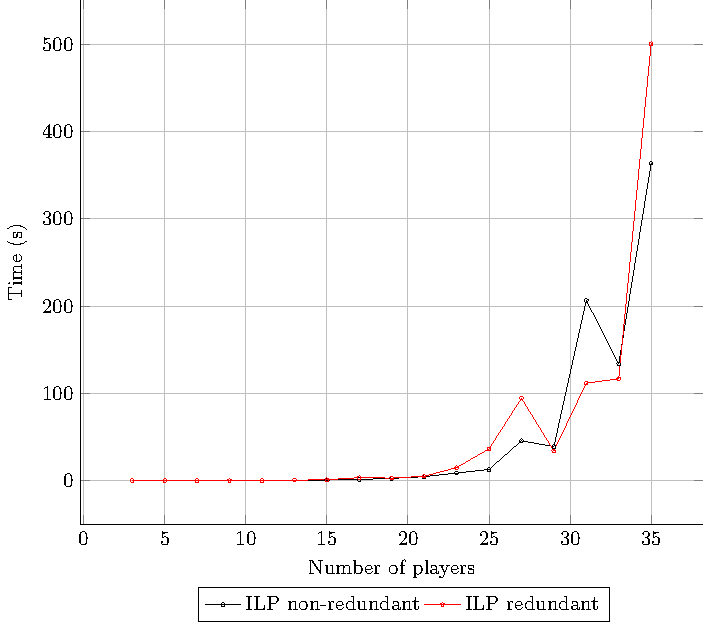
\includegraphics[width=\linewidth]{../plots/time_per_instance.pdf}
	\end{figure}
    \end{minipage}

\end{frame}

\section{Metaheuristics}
\subsection{Greedy algorithm}
\begin{frame}{\secname: \subsecname}
\begin{tcolorbox}[colback=gray!30, colframe=Veronablue, arc=0pt, outer arc=0pt, title = \textbf{Greedy cost function}]
    \begin{equation*}
      q(c,day)= c.points\_per\_day[day]
    \end{equation*}
\end{tcolorbox}


\begin{algorithm}[H]
	\caption{Greedy algorithm} 
	\begin{algorithmic}[1]
	  \State Players $\leftarrow$ Set of Players
	  \State rests $\leftarrow$ \{\}
	    \For {day in 0..days}
	      \State playersToRest $\leftarrow$ filter Players(p) $|$ p.hasNotRested
	    \State sortedPlayers $\leftarrow$ sort playersToRest(p) by q(p,day) (DESC) 
        \State select p $\in$ sortedPlayers.first()
	      \State rests[day]\ $\leftarrow$\ p
	    \EndFor
	\end{algorithmic} 
\end{algorithm}
\end{frame}

\subsection{Local Search}
\begin{frame}{\secname: \subsecname}
\begin{algorithm}[H]
	\caption{Local Search} 
	\begin{algorithmic}[1]
    \For {i in 0..days}
    \State best\_swap\_points $\leftarrow$ 0
    \State best\_swap $\leftarrow$ i
      \For {j in 0..days}
        \State change = EvaluateRestSwap(i,j)
        \If{change $>$ best\_swap\_points}
          \State best\_swap\_points $\leftarrow$ change
          \State best\_swap $\leftarrow$ j
        \EndIf
      \EndFor
      \State rests[i] $\leftrightarrow$ rests[best\_swap]
		\EndFor
	\end{algorithmic} 
\end{algorithm}



\end{frame}

\subsection{GRASP}
\begin{frame}{\secname: \subsecname}
\begin{algorithm}[H]
    \caption{constructRCL(day)} 
    \label{rcl}
    \begin{algorithmic}[1]
	\State $q_{max} \leftarrow $ sortedPlayers.first().points[d]
	\State $q_{min} \leftarrow$ sortedPlayers.last().points[d]
	\State $RCL_{max}$ $\leftarrow$ $\{p \in sortedPlayers\ |\ p.points[d] >= q_{max} - \alpha \cdot (q_{max} - q_{min})\}$
    \end{algorithmic} 
\end{algorithm}




\begin{algorithm}[H]
	\caption{GRASP} 
	\begin{algorithmic}[1]
	  \State rests $\leftarrow$ \{\}
	    \For {day in 0..days}
        \State playersToRest $\leftarrow$ filter Players(p) $|$ p.hasNotRested
        \State sortedPlayers $\leftarrow$ sort playersToRest(p) by q(p,day) (DESC)
	      \State RCL $\leftarrow$ constructRCL(day)
	      \State select p $\in$ RCL randomly
	      \State rests[day]\ $\leftarrow$\ p
	    \EndFor
	\end{algorithmic} 
\end{algorithm}
\end{frame}

\subsubsection{Parameter tuning}
\begin{frame}{\subsecname: \subsubsecname}

    \begin{minipage}{0.44\textwidth}
	\begin{itemize}
	    \item Figure shows the arithmetic mean error with respect to the optimal solution for each of the instances.
      \item We keep the smallest alpha that gives the minimum mean error.
	\end{itemize}
    \end{minipage}
    \hfill
    \begin{minipage}{0.52\textwidth}
	\centering
	\begin{figure}[H]
	    \centering
	    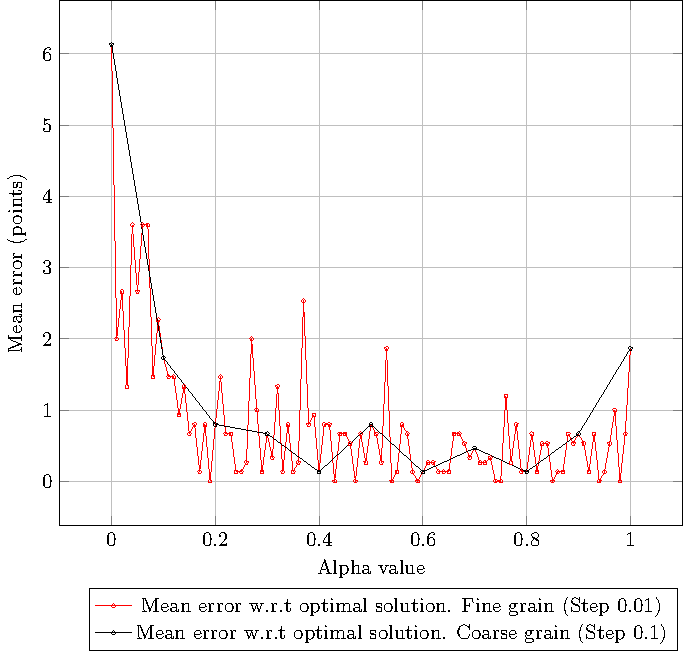
\includegraphics[width=\linewidth]{../plots/error.pdf}
	    \label{fig:error}
	\end{figure}
    \end{minipage}
\end{frame}

\section{Results}
\subsection{Time}
\begin{frame}{\secname: \subsecname}
    \begin{minipage}{0.44\textwidth}
	\begin{itemize}
	    \item Greedy and Local Search need approximately same time to reach the solution. They're fastest but their quality of the solution is too low.
	    \item GRASP sacrifices some runtime performance to improve the quality of the solution.
      \item ILPs obtain the optimal solution at cost of being several orders of magnitude slower due to the complexity of creating valid pairings.
      \item ILP rest obtains the optimal solution just computing the rest day for each player. It is not much slower than GRASP and for large instances it can be even faster.
	\end{itemize}
    \end{minipage}
    \hfill
    \begin{minipage}{0.52\textwidth}
	\centering
	\begin{figure}[H]
	    \centering
	    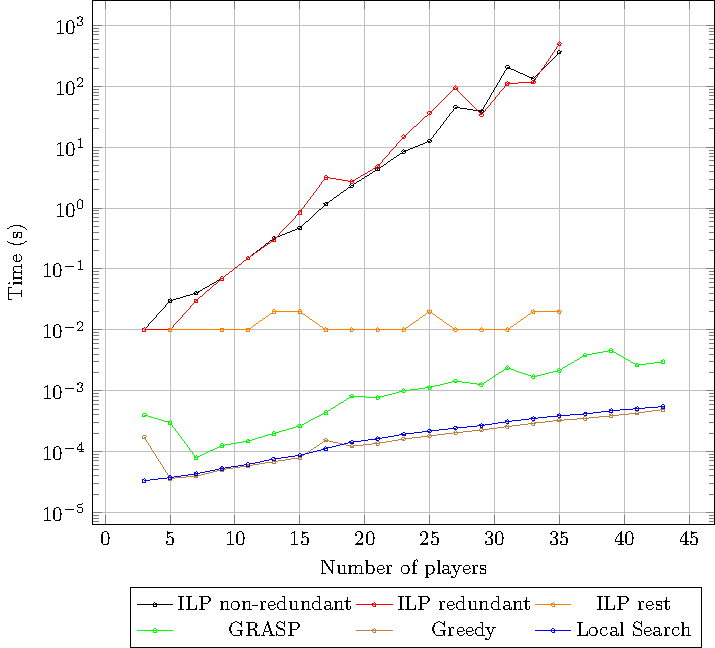
\includegraphics[width=\linewidth]{../plots/times.pdf}
	\end{figure}
    \end{minipage}
\end{frame}

\subsection{Quality of solutions}
\begin{frame}{\secname: \subsecname}
    \begin{minipage}{0.44\textwidth}
	\begin{itemize}
	    \item Greedy offers the worst solution for every instance
	    \item Greedy + Local Search improves the quality of the solution taking practically the same time as Greedy.
      \item GRASP commonly reachs the optimal solution, having a great improvement over Local  Search.
	\end{itemize}
    \end{minipage}
    \hfill
    \begin{minipage}{0.52\textwidth}
	\centering
	\begin{figure}[H]
	    \centering
	    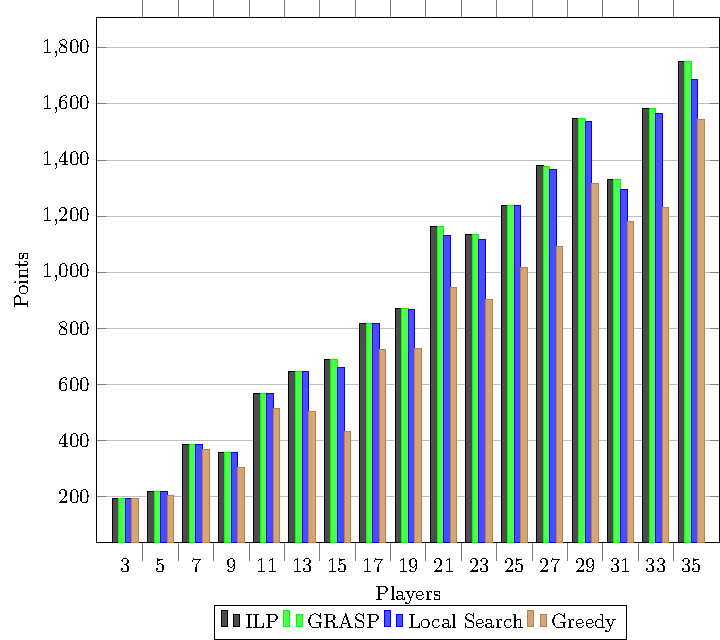
\includegraphics[width=\linewidth]{../plots/solutions.pdf}
	\end{figure}
    \end{minipage}
\end{frame}



%\subsection{Ruidos a filtrar}
%\begin{frame}{\secname: \subsecname}
%    %\begin{figure}[H]
%	%\begin{subfigure}{0.3\textwidth}
%	    %\includegraphics[width=\linewidth]{imagenes/ruidogaussiano_1.jpg}
%	    %\caption{Original}
%	%\end{subfigure}
%	%\hfill
%	%\begin{subfigure}{0.3\textwidth}
%	    %\includegraphics[width=\linewidth]{imagenes/ruidogaussiano_2.jpg}
%	    %\caption{Ruido gaussiano}
%	%\end{subfigure}
%	%\hfill
%	%\begin{subfigure}{0.3\textwidth}
%	    %\includegraphics[width=\linewidth]{imagenes/ruidoimpulsivo_1.jpg}
%	    %\caption{Ruido impulsivo}
%	%\end{subfigure}
%	%\caption{Ruidos a filtrar y sus efectos visuales}
%    %\end{figure}
%\end{frame}
%
%\section{Marco Teórico}
%\subsection{Algoritmo}
%\begin{frame}{\secname: \subsecname}
%    \begin{minipage}{0.45\textwidth}
%	Primero, un poco de notación:
%
%	\begin{itemize}
%	    \item $x_i$ se refiere al pixel que está siendo filtrado
%	    \item $x^j$ se refiere a cualquier pixel dentro de la ventana
%		de filtrado
%	\end{itemize}
%
%	Trabajaremos con los $q$ vecinos más similares a $x_i$
%    \end{minipage}\hfill
%    \begin{minipage}{0.45\textwidth}
%	%\begin{figure}[H]
%	    %\centering
%	    %\includegraphics[width=\linewidth]{../archivos/tests/window.pdf}
%	    %\caption{Ventana de filtrado. Ejemplo de dimensiones 3x3}
%	%\end{figure}
%    \end{minipage}
%\end{frame}
%
%\begin{frame}{\secname: \subsecname}
%    \center{
%	Caracterización de los ruidos gaussianos e impulsivos.
%    }
%
%    \begin{minipage}{0.45\textwidth}
%	%\begin{figure}[H]
%	    %\centering
%	    %\includegraphics[width=0.7\linewidth]{../archivos/ventana.pdf}
%	%\end{figure}
%	Grado de impulsividad determinado por la métrica $\displaystyle \text{ROAD}_m = \sum_{j=1}^{m}d(x_i, x^j) $
%    \end{minipage}\hfill
%    \begin{minipage}{0.45\textwidth}
%	%\begin{figure}[H]
%	    %\centering
%	    %\includegraphics[width=\linewidth]{../archivos/similaritydegree.pdf}
%	%\end{figure}
%	Tres grados de semejanza: alta, media y baja. Dependiente de
%	la distancia entre píxeles $d(x_i, x^j)$.
%    \end{minipage}
%\end{frame}
%
%
%\begin{frame}{\secname: \subsecname}
%    \begin{minipage}{0.4\textwidth}
%	\begin{itemize}
%	    \item Reglas difusas 
%
%		\begin{enumerate}
%		    \item $\dots$
%		    \item \textbf{SI} ($x^j$ no es impulsivo \textbf{Y} $x_i$ es impulsivo \textbf{Y} 
%			la semejanza entre $x^j$ y $x_i$ es moderada) \textbf{ENTONCES} $\omega_j$ 
%			es un peso \textbf{moderado}.
%		    \item $\dots$
%		\end{enumerate}
%	    \item Defuzzificación mediante el centro de gravedad
%	\end{itemize}
%
%    \end{minipage}\hfill
%    \begin{minipage}{0.6\textwidth}
%	\begin{center}
%	\scalebox{0.55}{
%	    \begin{algorithm}[H] %or another one check
%	     \caption{Filtro difuso secuencial}
%		\KwData{Imagen ruidosa $I$, parámetros $n, q, m, p_1, p_2, p_3, p_4$}
%		\KwResult{Imagen filtrada $I^{\prime}$}
%
%		Imagen $I_0 = I$\\
%		\For{Iteración $\  it = 1,\ldots$}{
%			Imagen $I_{it} = I_{it-1}$\\
%			\For{$x_i$ pixel $\in$ ${I_{it}}$}{
%			    Tomar la ventana $W$ $n \times n$ centrada en $x_i$\\
%			    %Tomar la $n \times n$ filtering window $W$ with central pixel $x_i$\\
%			    \textbf{\underline{Cálculo del grado de impulsividad}}\\
%				\Indp
%				Calcular $\mu (x_i)$\\
%				\Indm
%			    \textbf{\underline{Cálculo del grado de semejanza}}\\
%				\Indp
%				Ordenar los píxeles $  x^j \in W$ según $d(x_i, x^j)$\\
%				Seleccionar los $q$ píxeles mas cercanos $x^1,\ldots,x^q$\\
%				\For {$ j = 1,\ldots, q$}{
%				    Calcular $\mu_H (x_i, x^j), \mu_L (x_i, x^j), \mu_H (x_i , x^j),$
%				}
%				\Indm
%			    %\textbf{\underline{Computation of averaging weights by defuzzyficattion}}}
%			    \textbf{\underline{Cálculo de los pesos mediante defuzzificación}}\\
%				\Indp
%				\For{$ j = 1,\ldots, q$}{
%				    %Compute certainty degree of the antecedents of fuzzy rules for  $x^j$\\
%				    Calcular las reglas difusas para \{$x_i, x^j$\}\\
%				    Calcular el peso $w_j$ correspondiente a $x^j$ mediante COG\\
%				}
%				\Indm
%			    \textbf{\underline{Cálculo del nuevo valor para $x_i$}}\\
%				\Indp
%				$\displaystyle \hat{x}_i = \frac{\sum_{j=1}^{q} \omega_j \cdot x^{j}}{\sum_{j=1}^{q} \omega_j}$\\
%				\Indm
%			}
%		}
%		\label{algoritmo_filtro_secuencial}
%	    \end{algorithm}
%	}
%	\end{center}
%    \end{minipage}
%\end{frame}
%
%%\begin{frame}{\secname: \subsecname}
%    %\begin{center}
%    %\scalebox{0.6}{
%	%\begin{algorithm}[H] %or another one check
%	 %\caption{Filtro difuso secuencial}
%	    %\KwData{Imagen ruidosa $I$, parámetros $n, q, m, p_1, p_2, p_3, p_4$}
%	    %\KwResult{Imagen filtrada $I^{\prime}$}
%
%	    %Imagen $I_0 = I$\\
%	    %\For{Iteración $\  it = 1,\ldots$}{
%		    %Imagen $I_{it} = I_{it-1}$\\
%		    %\For{$x_i$ pixel $\in$ ${I_{it}}$}{
%			%Tomar la ventana $W$ $n \times n$ centrada en $x_i$\\
%			%%Tomar la $n \times n$ filtering window $W$ with central pixel $x_i$\\
%			%\textbf{\underline{Cálculo del grado de impulsividad}}\\
%			    %\Indp
%			    %Calcular $\mu (x_i)$\\
%			    %\Indm
%			%\textbf{\underline{Cálculo del grado de semejanza}}\\
%			    %\Indp
%			    %Ordenar los píxeles $  x^j \in W$ según $d(x_i, xj)$\\
%			    %Seleccionar los $q$ píxeles mas cercanos $x^1,\ldots,x^q$\\
%			    %\For {$ j = 1,\ldots, q$}{
%				%Calcular $\mu_H (x_i, x^j), \mu_L (x_i, x^j), \mu_H (x_i , x^j),$
%			    %}
%			    %\Indm
%			%%\textbf{\underline{Computation of averaging weights by defuzzyficattion}}}
%			%\textbf{\underline{Cálculo de los pesos mediante defuzzificación}}\\
%			    %\Indp
%			    %\For{$ j = 1,\ldots, q$}{
%				%%Compute certainty degree of the antecedents of fuzzy rules for  $x^j$\\
%				%Calcular las reglas difusas para \{$x_i, x^j$\}\\
%				%Calcular el peso $w_j$ correspondiente a $x^j$ mediante COG\\
%			    %}
%			    %\Indm
%			%\textbf{\underline{Cálculo del nuevo valor para $x_i$}}\\
%			    %\Indp
%			    %$\displaystyle \hat{x}_i = \frac{\sum_{j=1}^{q} \omega_j \cdot x^{j}}{\sum_{j=1}^{q} \omega_j}$\\
%			    %\Indm
%		    %}
%	    %}
%	    %\label{algoritmo_filtro_secuencial}
%	%\end{algorithm}
%    %}
%    %\end{center}
%
%%\end{frame}
%
%
%\section{Implementación}
%    %\begin{frame}{\secname : \subsecname}
%	%Consideraciones generales
%
%	%Secuencial
%
%	%Paralela
%
%	%Distribuida
%    %\end{frame}
%%\subsection{Consideraciones generales}
%%\begin{frame}{\secname : \subsecname}
%    %Evitar código spaguetti, clases representando ventanas, imágenes sobre un array plano, todo código desde 0 para tener
%    %más control...
%%\end{frame}
%
%\subsection{Versión secuencial}
%\begin{frame}{\secname : \subsecname}
%    \center{
%	Cálculo del centro de gravedad mediante métodos geométricos.
%    }
%    \begin{minipage}{0.505\textwidth}
%	%\begin{figure}[H]
%	    %\includegraphics[width=\textwidth]{../archivos/cogcomputation}
%	    %\caption{Centro de gravedad a obtener por cada $x_i, x_j \in W$}
%	%\end{figure}
%    \end{minipage}
%    \hfill
%    \begin{minipage}{0.46\textwidth}
%	%\begin{figure}[H]
%	    %\includegraphics[width=\textwidth]{../archivos/benchmarks/calculateweight.pdf}
%	    %\caption{Aceleración obtenida gracias al cálculo geométrico}
%	%\end{figure}
%    \end{minipage}
%\end{frame}
%
%\begin{frame}{\secname: \subsecname}
%    %\begin{minipage}{0.60\textwidth}
%	%\begin{figure}[H]
%	    %\includegraphics[width=\textwidth]{../archivos/pgmwindowcreation.pdf}
%	    %\caption{}
%	%\end{figure}
%    %\end{minipage}
%    %\hfill
%    %\begin{minipage}{0.274\textwidth}
%	%\begin{figure}[H]
%	    %\includegraphics[width=\textwidth]{../archivos/pgmwindow.pdf}
%	    %\caption{Gestión de las ventanas de manera transparente al\\ desarrollador}
%	%\end{figure}
%    %\end{minipage}
%
%    \begin{figure}[H]
%	\hspace{0.05\textwidth}
%	%\begin{subfigure}{0.3\textwidth}
%	    %\includegraphics[width=\textwidth]{../archivos/pgmwindow.pdf}
%	    %\caption{Ventanas que sobrepasan los límites de la imagen a filtrar}
%	%\end{subfigure}
%	\hfill
%	%\begin{subfigure}{0.4\textwidth}
%	    %\includegraphics[width=\textwidth]{../archivos/pgmwindowcreation.pdf}
%	    %\caption{Ajuste automático. $W \rightarrow W'$}
%	%\end{subfigure}
%	\hspace{0.05\textwidth}
%	\caption{Gestión de las ventanas de filtrado transparente al desarrollador}
%    \end{figure}
%
%\end{frame}
%
%\begin{frame}{\secname: \subsecname}
%    \begin{minipage}{0.44\textwidth}
%	La implementación inicial ingenua podía llegar a calcular el grado
%	de impulsividad de cada pixel en numerosas ocasiones. Por ello introdujimos
%	un <<almacén>> de grados de impulsividad para evitar este problema. 
%    \end{minipage}
%    \hfill
%    \begin{minipage}{0.50\textwidth}
%	%\begin{figure}[H]
%	    %\includegraphics[width=\textwidth, left]{../archivos/secoptimizada.pdf}
%	%\end{figure}
%    \end{minipage}
%\end{frame}
%
%\subsection{Versión en memoria compartida}
%\begin{frame}{\secname : \subsecname}
%    \begin{minipage}{0.50\textwidth}
%	Paralelización del núcleo de la aplicación mediante directivas 
%	de \textcolor[HTML]{00737D}{OpenMP}. 
%	\begin{itemize}
%	    \item Paralelización del tratamiento de la imagen. 
%	    \item Almacenamiento local para cada hilo (TLS)
%	    \item Sincronización sin cerrojos
%	\end{itemize}
%    \end{minipage}\hfill
%    \begin{minipage}{0.47\textwidth}
%	%\begin{figure}[H]
%	    %\includegraphics[width=\textwidth, left]{../archivos/figure4_old.png}
%	    %\caption{La paralelización actúa a nivel de subdominio $\Omega_i$}
%	%\end{figure}
%    \end{minipage}
%\end{frame}
%
%\subsection{Versión distribuida}
%\begin{frame}{\secname : \subsecname}
%    \begin{minipage}{0.44\textwidth}
%	Desarrollada utilizando MPI.
%
%	\vspace{0.5cm}
%
%	Tamaño de ventana $n = 2\omega + 1$
%
%
%	\begin{itemize}
%	    \item $\Omega_i$: Región a \textbf{filtrar} por el nodo $i$
%	    \item $\Omega_i^\omega$: Región a \textbf{necesaria} para el nodo $i$
%	    \item \testclr{black!25!}{Solapamiento} $\rightarrow$ \textbf{Comunicación}
%	\end{itemize}
%
%	\begin{tcolorbox}[colback=gray!30, colframe=Veronablue, title = \textbf{Propuesta}]
%	    Esquema de iteraciones locales. En lugar de comunicar cada iteración, hacerlo
%	    cada $x$ iteraciones.
%	\end{tcolorbox}
%    \end{minipage}\hfill
%    \begin{minipage}{0.55\textwidth}
%
%	%\noindent\begin{figure}[H]
%	    %\includegraphics[width=\textwidth, left]{../archivos/domaindecomposition.pdf}
%	    %\caption{Descomposición del trabajo para 3 nodos}
%	    %\label{figure5}
%	%\end{figure}
%    \end{minipage}
%\end{frame}
%
%\section{Rendimiento}
%
%\subsection{Equipos de pruebas}
%\begin{frame}{\secname : \subsecname}
%    %\begin{minipage}[t]{0.49\textwidth}
%
%	%\begin{tcolorbox}[colback=gray!40, colframe=Veronablue!90, title = \faDesktop \ Equipo 1. Ordenador personal]
%	    %\begin{itemize}
%		%\itemsep0.2em
%		%\setlength{\itemindent}{-1em}
%		%\item (x1) AMD Ryzen 2700X (8C / 16T), 16GB RAM DDR4 3200MT/s
%		%\item ArchLinux. Kernel 5.16.12 
%		%\item GCC 11.2.0
%	    %\end{itemize}
%	%\end{tcolorbox}
%	%\vfill
%    %\end{minipage}\hfill
%    %\begin{minipage}[t]{0.49\textwidth}
%	%%\vspace{1.435cm}
%	%\begin{tcolorbox}[colback=gray!40, colframe=Veronablue!90, title = \faDesktop \  Equipo 2. Cluster del IUII]
%	    %%\vspace{.95cm}
%	    %\begin{itemize}
%		%\itemsep0.2em
%		%\setlength{\itemindent}{-1em}
%		%\item (2x) CPU Intel Xeon X 5660 (6C/12T), 48GB RAM DDR3 1333MT/s
%		%\item CentOS 7. Kernel 3.10.0
%		%\item GCC 7.5.0
%		%\item OpenMPI 4.0.2
%	    %\end{itemize}
%	%\end{tcolorbox}
%	%\vfill
%    %\end{minipage}
%
%    \begin{multicols}{2}
%	\begin{tcolorbox}[colback=gray!30, colframe=Veronablue, title = \faDesktop \ Equipo 1. Ordenador personal,
%	   height=4cm ]
%	    \begin{itemize}
%		\itemsep0.2em
%		\setlength{\itemindent}{-1em}
%		\item (x1) AMD Ryzen 2700X (8C / 16T), 16GB RAM DDR4 3200MT/s
%		\item ArchLinux. Kernel 5.16.12 
%		\item GCC 11.2.0
%	    \end{itemize}
%	\end{tcolorbox}
%	\columnbreak
%
%	\begin{tcolorbox}[colback=gray!30, colframe=Veronablue, title = \faDesktop \  Equipo 2. Cluster del IUII, height=4cm]
%	    %\vspace{.95cm}
%	    \begin{itemize}
%		\itemsep0.2em
%		\setlength{\itemindent}{-1em}
%		\item (2x) CPU Intel Xeon X 5660 (6C/12T), 48GB RAM DDR3 1333MT/s
%		\item CentOS 7. Kernel 3.10.0
%		\item GCC 7.5.0
%		\item OpenMPI 4.0.2
%	    \end{itemize}
%	\end{tcolorbox}
%
%    \end{multicols}
%\end{frame}
%
%\subsection{Versión en memoria compartida}
%    \begin{frame}{\secname : \subsecname}
%	\begin{minipage}{0.25\textwidth}
%	    Rendimiento {\color{ao}óptimo} en el Equipo 1.
%
%	    \vspace{0.5cm}
%
%	    Rendimiento {\color{alizarin}subóptimo} en el Equipo 2.
%	    \begin{itemize}
%		\item Nodos dual-socket
%		\item Compilador más anticuado
%	    \end{itemize}
%
%	\end{minipage}
%	\hfill
%	\begin{minipage}{0.70\textwidth}
%	    %\begin{figure}[H]
%		%\includegraphics[width=\textwidth]{../archivos/benchmarks/openmp_impl_bar.pdf}
%		%\caption{Benchmark medido en el Equipo 1}
%	    %\end{figure}
%	\end{minipage}
%    \end{frame}
%\subsection{Versión distribuida}
%    \begin{frame}{\secname : \subsecname}
%
%	\begin{minipage}{0.49\textwidth}
%	    %\begin{figure}[H]
%		%\includegraphics[width=\textwidth]{../archivos/tests/mpi/escalado_nodosmpi.pdf} 
%	    %\end{figure}
%	\end{minipage}\hfill
%	\begin{minipage}{0.49\textwidth}
%	    %\begin{figure}[H]
%		%\includegraphics[width=\textwidth]{../archivos/tests/mpi/escalado_general.pdf} 
%	    %\end{figure}
%	\end{minipage}
%    \end{frame}
%\subsubsection{Esquema de iteraciones locales}
%    \begin{frame}{\secname : \subsecname}
%
%	\begin{minipage}{0.45\textwidth}
%	\begin{itemize}
%	    \item La eficiencia combinada se ve lastrada por el rendimiento paralelo en los
%		  equipos del clúster. 
%	    %\item Bastante variabilidad de resultados a la hora de medir en el clúster.
%	\end{itemize}
%
%	\vspace{1cm}
%
%	\begin{itemize}
%	    \item El esquema de iteraciones locales supone una aceleración cercana al 
%		\textbf{12\%} sin pérdida de calidad de filtrado.
%	\end{itemize}
%	\end{minipage}\hfill
%	\begin{minipage}{0.50\textwidth}
%	    %\begin{figure}[H]
%		%\includegraphics[width=\textwidth]{../archivos/tests/mpi/iteracionesinternas.pdf} 
%	    %\end{figure}
%	\end{minipage}
%    \end{frame}
%
%\section{Calidad de filtrado}
%\subsection{Métricas numéricas}
%    \begin{frame}{\secname : \subsecname \ I}
%	\begin{table}[H] 
%	\centering
%	\begin{tabular}{c@{\quad}cc@{\quad}cc@{\quad}cc}
%	\toprule
%	\multicolumn{1}{c}{\rule{0pt}{12pt} }&\multicolumn{6}{c}{MAE}\\[2pt]
%	\multicolumn{1}{c}{\rule{0pt}{12pt} }&\multicolumn{2}{c}{Vista axial}&\multicolumn{2}{c}{Vista sagital}&\multicolumn{2}{c}{Vista coronal}\\[2pt]
%	\multicolumn{1}{c}{\rule{0pt}{12pt}Ruido}& Ruidosa & Filtrada & Ruidosa & Filtrada & Ruidosa & Filtrada\\[2pt]                   
%	\midrule
%	$\sigma=5, \ p=0.05$ & 13.19  &  4.32 &   8.54      &  2.60     &  9.20      & 2.98     \\
%	$\sigma=10, \ p=0.1$ & 21.29  &  5.97 &  14.28      &  3.61     &  15.37     & 4.07     \\
%	$\sigma=20, \ p=0.2$ & 35.65  &  8.26 &  24.87      &  5.91     &  26.64     & 6.47     \\
%	$\sigma=30, \ p=0.3$ & 50.03  & 13.02 &  34.84      &  9.08     &  37.29     & 9.81     \\
%	\bottomrule
%	\end{tabular}
%	\caption{Valores mínimos de MAE en las imágenes contaminadas con los distintos ruidos gaussiano e impulsivos}
%	\end{table}
%    \end{frame}
%
%    \begin{frame}{\secname : \subsecname \ II}
%	\begin{table}[H] 
%	\centering
%	\begin{tabular}{c@{\quad}cc@{\quad}cc@{\quad}cc}
%	\toprule
%	\multicolumn{1}{c}{\rule{0pt}{12pt} }&\multicolumn{6}{c}{PSNR}\\[2pt]
%	\multicolumn{1}{c}{\rule{0pt}{12pt} }&\multicolumn{2}{c}{Vista axial}&\multicolumn{2}{c}{Vista sagital}&\multicolumn{2}{c}{Vista coronal}\\[2pt]
%	\multicolumn{1}{c}{\rule{0pt}{12pt}Ruido}& Ruidosa & Filtrada & Ruidosa & Filtrada & Ruidosa & Filtrada\\[2pt]                   
%	\midrule
%	$\sigma=5, \ p=0.05$ & 19.03  & 34.57 &  18.85  & 34.81 & 19.21  & 34.32 \\
%	$\sigma=10, \ p=0.1$ & 16.06  & 32.22 &  15.86  & 32.53 & 16.13  & 32.03 \\
%	$\sigma=20, \ p=0.2$ & 12.98  & 29.53 &  12.82  & 28.80 & 13.07  & 28.46 \\
%	$\sigma=30, \ p=0.3$ & 11.17  & 25.80 &  11.02  & 25.24 & 11.25  & 25.06 \\
%	\bottomrule
%	\end{tabular}
%	\caption{Valores máximos de PSNR en las imágenes contaminadas con los distintos ruidos gaussiano e impulsivos}
%	\label{psnr}
%	\end{table}
%    \end{frame}
%
%
%\subsection{Calidad visual}
%\begin{frame}{\secname : \subsecname}
%    %\begin{figure}[H]
%	%\begin{subfigure}{0.328\textwidth}
%	    %\includegraphics[width=\linewidth]{../archivos/imagenes/coronal_g10_i01.pgm.png}
%	    %\caption{Contaminada $\sigma=10,\rho=0.1$}
%	%\end{subfigure}
%	%\begin{subfigure}{0.328\textwidth}
%	    %\includegraphics[width=\linewidth]{../archivos/imagenes/coronal_g10_i01.pgm.filtered.pgm.png}
%	    %\caption{Filtrada}
%	%\end{subfigure}
%	%\begin{subfigure}{0.328\textwidth}
%	    %\includegraphics[width=\linewidth]{../archivos/coronal.png}
%	    %\caption{Original}
%	%\end{subfigure}
%	%\caption{Vista coronal contaminada, filtrada y original}
%    %\end{figure}
%\end{frame}
%
%%%%%%%%%%%%%%%%%%%%%%%%%%%%%%%%%%%%%%%%%%%%%%%%%%%%%%%%%%%%%%%%%%%%%%%%%%%%%%%%%%%%%
%%%%%%%%%%%%%%%%%%%%%%%%%%%%%%%%%%%%%%%%%%%%%%%%%%%%%%%%%%%%%%%%%%%%%%%%%%%%%%%%%%%%%
%
%%\begin{frame}{\secname : \subsecname}
%    %\begin{figure}[H]
%	%\includegraphics[width=0.5\linewidth]{../archivos/imagenes/coronal_g10_i01.pgm.png}
%	%\caption{\scriptsize{Contaminada $\sigma=10,\rho=0.1$}}
%    %\end{figure}
%%\end{frame}
%
%%\begin{frame}{\secname : \subsecname}
%    %\begin{figure}[H]
%	%\begin{subfigure}{0.45\textwidth}
%	    %\includegraphics[width=\linewidth]{../archivos/imagenes/coronal_g10_i01.pgm.filtered.pgm.png}
%	    %\caption{Filtrada}
%	%\end{subfigure}
%	%\hfill
%	%\begin{subfigure}{0.45\textwidth}
%	    %\includegraphics[width=\linewidth]{../archivos/coronal.png}
%	    %\caption{Original}
%	%\end{subfigure}
%	%\caption{Vista coronal contaminada, filtrada y original}
%    %\end{figure}
%%\end{frame}
%
%
%%%%%%%%%%%%%%%%%%%%%%%%%%%%%%%%%%%%%%%%%%%%%%%%%%%%%%%%%%%%%%%%%%%%%%%%%%%%%%%%%%%%%
%%%%%%%%%%%%%%%%%%%%%%%%%%%%%%%%%%%%%%%%%%%%%%%%%%%%%%%%%%%%%%%%%%%%%%%%%%%%%%%%%%%%%
%
%
%\section{Conclusión}
%\begin{frame}{\secname}
%    \textbf{Resultados:}
%    \begin{itemize}
%	\item Alta eficiencia de la implementación paralela 
%	    % Comentar que es con el número mayor de nodos.
%	    \begin{itemize}
%		\item $> 85\%$ Equipo 1
%		\item $> 96\%$ Equipo 2
%	    \end{itemize}
%	\item Alta eficiencia de la implementación distribuida. $> 82\%$
%	      con 20 nodos.
%	\item Calidad de filtrado notable.
%    \end{itemize}
%    \textbf{Líneas futuras:}
%    \begin{itemize}
%	\item Implementación con primitivas MPI no bloqueantes.
%	\item Desarrollar una versión acelerada por GPU.
%    \end{itemize}
%\end{frame}
%
%\begin{frame}{\secname}
%    \begin{minipage}{0.54\textwidth}
%	\huge{Gracias por su atención.}
%    \end{minipage}\hfill
%    \begin{minipage}{0.32\textwidth}
%	%\noindent\begin{figure}[H]
%	    %\includegraphics[width=\textwidth, left]{portada.pdf}
%	%\end{figure}
%    \end{minipage}
%
%\end{frame}
%
%
%%\section{Aclaraciones}
%%\subsection{Lógica difusa}
%\begin{frame}[noframenumbering]{Aclaraciones}
%    \begin{minipage}{0.55\textwidth}
%    \begin{itemize}
%	\item Valores lógicos $\{0, 1\} \rightarrow [0, 1]$
%	\item Pertenencia a conjuntos definida por funciones 
%	\item Operadores lógicos  
%		%\item $\{A \land B, A \lor B\} \rightarrow \{A \cdot B, A + B - A \cdot B\}$ 
%	    \begin{itemize}
%		\item $\{A \land B\} \rightarrow \{A \cdot B\}$ 
%		\item $\{A \lor B\} \rightarrow \{A + B - A \cdot B\}$ 
%	    \end{itemize}
%	\item Reglas difusas
%	\item Defuzzificación
%    \end{itemize}
%    \end{minipage}\hfill
%    \begin{minipage}{0.4\textwidth}
%	%\begin{figure}[H]
%	    %\centering
%	    %\includegraphics[width=\textwidth]{../archivos/similaritydegree}
%	    %\caption{Grado de semejanza para un pixel $x^j$ en función de $d(x_i, x^j)$}
%	%\end{figure}
%
%    \end{minipage}
%\end{frame}
%\begin{frame}[noframenumbering]{Aclaraciones II}
%    \begin{minipage}{0.55\textwidth}
%	\begin{itemize}
%	    \item Caracterización de la impulsividad y la semejanza entre píxeles dentro de la ventana de filtrado.
%	    \item Reglas difusas 
%
%		\begin{enumerate}
%		    \item $\dots$
%		    \item \textbf{SI} ($x^j$ no es impulsivo \textbf{Y} $x_i$ es impulsivo \textbf{Y} 
%			la semejanza entre $x^j$ y $x_i$ es moderada) \textbf{ENTONCES} $\omega_j$ 
%			es un peso \textbf{moderado}.
%		    \item $\dots$
%		\end{enumerate}
%	    \item Defuzzificación mediante el centro de gravedad
%	\end{itemize}
%
%    \end{minipage}\hfill
%    \begin{minipage}{0.4\textwidth}
%	%\begin{figure}[H]
%	    %\includegraphics[width=\textwidth]{../archivos/membershipfunctions}
%	    %\caption{Funciones de membresía $\eta_H (\omega_j),\ \eta_M (\omega_j),$ y $\eta_L
%		    %(\omega_j)$ junto a $K_{L}, K_{M}, K_{H}$ correspondientes a las 
%		    %reglas difusas \{1, 2, 3\} respectivamente para determinados píxeles $x_{i}$ y $x^j$}
%	%\end{figure}
%
%    \end{minipage}
%\end{frame}

%\begin{frame}[noframenumbering]{\secname}

%\end{frame}


\end{document}
